% ============================================================
%  Rate-Distortion Comparison — Sensor-Based vs. Traditional Compressors
%  ISABEL CLOUDf48  ds=10  (50x50/level)
%  Compile: pdflatex slides_rd_comparison.tex  (run twice)
%  Requires: beamer-theme-metropolis  (tlmgr install beamer-theme-metropolis)
%  Figures must be in the same directory as this .tex file.
% ============================================================
\documentclass[aspectratio=169, 11pt]{beamer}

\usetheme{metropolis}

% ── packages ────────────────────────────────────────────────
\usepackage{booktabs}
\usepackage{colortbl}
\usepackage{amsmath, amssymb}
\usepackage{graphicx}
\usepackage{xcolor}
\usepackage{tikz}
\usepackage[protrusion=true, expansion=false]{microtype}
\usepackage[T1]{fontenc}
\usetikzlibrary{arrows.meta}

\graphicspath{{./}}

% ── colour palette ──────────────────────────────────────────
\definecolor{cnavy}{HTML}{0D2137}
\definecolor{cteal}{HTML}{1A6B8A}
\definecolor{cice}{HTML}{D6EBF5}
\definecolor{camber}{HTML}{F0A500}
\definecolor{cgreen}{HTML}{1D8A5E}
\definecolor{cred}{HTML}{C0392B}
\definecolor{cmuted}{HTML}{5A7385}

% ── metropolis overrides ────────────────────────────────────
\setbeamercolor{normal text}{fg=cnavy, bg=white}
\setbeamercolor{frametitle}{bg=cnavy, fg=white}
\setbeamercolor{title separator}{fg=cteal}
\setbeamercolor{progress bar}{fg=cteal, bg=cice}
\setbeamercolor{alerted text}{fg=camber}
\setbeamercolor{block title}{bg=cice, fg=cnavy}
\setbeamercolor{block body}{bg=cice!40, fg=cnavy}
\setbeamercolor{itemize item}{fg=cteal}
\setbeamercolor{itemize subitem}{fg=cmuted}
\setbeamercolor{enumerate item}{fg=cteal}
\setbeamerfont{frametitle}{size=\large, series=\bfseries}
\setbeamerfont{block title}{series=\bfseries, size=\small}
\setbeamerfont{block body}{size=\small}

% ── macros ───────────────────────────────────────────────────
\newcommand{\tightarrow}{%
  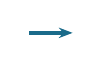
\begin{tikzpicture}[baseline=-0.5ex]
    \draw[-{Stealth[length=5pt]}, line width=1.2pt, color=cteal] (0,0)--(0.55,0);
  \end{tikzpicture}}

% ── title info ───────────────────────────────────────────────
\title{Rate-Distortion Comparison}
\subtitle{Sensor-Based Methods vs.\ SZ2 and ZFP on ISABEL Hurricane Data}
\author{Jessie Chen}
\institute{Argonne National Laboratory}
\date{July 2026}

% ============================================================
\begin{document}
% ============================================================

% ── SLIDE 1: Title ──────────────────────────────────────────
\maketitle

% ── SLIDE 2: Experimental Setup ─────────────────────────────
\begin{frame}{Experimental Setup}
\begin{columns}[T]

\begin{column}{0.48\textwidth}
  \textcolor{cteal}{\textbf{Dataset}}\vspace{0.15em}
  \begin{itemize}\setlength\itemsep{0.2em}\small
    \item ISABEL hurricane simulation — field: \textbf{CLOUDf}
    \item Shape: $100\!\times\!500\!\times\!500$, float32; $ds=10\;\to\;100\!\times\!50\!\times\!50$
    \item CR denominator = downsampled bytes; metrics at level 50
  \end{itemize}

  \vspace{0.35em}
  \textcolor{cteal}{\textbf{Shared quantization}}\vspace{0.15em}
  \begin{itemize}\setlength\itemsep{0.2em}\small
    \item \texttt{abs\_bound}: \texttt{logspace(-4,\,-0.5,\,8)}
    \item \texttt{bin\_width} $= 2\!\times\!\texttt{abs\_bound}/65536$ (matches SZ2)
    \item Huffman entropy estimate for all methods
  \end{itemize}
\end{column}

\begin{column}{0.48\textwidth}
  \textcolor{cteal}{\textbf{Six methods compared}}\vspace{0.2em}

  \begingroup
  \setbeamercolor{block title}{bg=cmuted!20, fg=cnavy}
  \setbeamercolor{block body}{bg=cmuted!10, fg=cnavy}
  \begin{block}{Traditional (baselines)}
    \scriptsize
    \textbf{SZ2} — Lorenzo predictor $\to$ quantize $\to$ Huffman $\to$ Zstd\\
    \textbf{ZFP} — block-floating-point transform, rate-controlled
  \end{block}
  \endgroup

  \vspace{0.3em}

  \begingroup
  \setbeamercolor{block title}{bg=cgreen!15, fg=cgreen}
  \setbeamercolor{block body}{bg=cgreen!5, fg=cnavy}
  \begin{block}{Sensor-based (this work)}
    \scriptsize
    \textbf{DEIM-2D} — per-level SVD, Q-DEIM sensors (lat, lon)\\
    \textbf{T-DEIM} — 3-D POD basis, sensors in full volume\\
    \textbf{Kriging-2D} — per-level GP (Matérn-3/2), GKS sensors\\
    \textbf{MultiGP} — ICM/LMC joint (CLOUDf $+$ QVAPORf)
  \end{block}
  \endgroup
\end{column}

\end{columns}
\end{frame}

% ── SLIDE 3: Compression Pipeline ───────────────────────────
\begin{frame}{Compression Pipelines at a Glance}
\small

\vspace{0.2em}
\renewcommand{\arraystretch}{1.15}
\scriptsize
\begin{tabular}{p{1.5cm}p{3.0cm}p{3.0cm}p{4.2cm}}
\toprule
\rowcolor{cnavy}
\textcolor{white}{\textbf{Method}} &
\textcolor{white}{\textbf{Prediction model}} &
\textcolor{white}{\textbf{Sensors / parameters}} &
\textcolor{white}{\textbf{Stored bytes}} \\
\midrule
SZ2
  & 3-D Lorenzo predictor
  & \textemdash
  & Huffman(quantized Lorenzo residuals) + raw outliers \\
\rowcolor{cice!40}
ZFP
  & Block floating-point
  & Rate (bpv)
  & Fixed-rate bit stream \\
DEIM-2D
  & Per-level 2-D SVD, $k$ modes
  & $k$ Q-DEIM sensors (lat, lon)
  & float16($\Phi$) + int32(sensors) + mean + float16(sensor vals) + Huffman(residuals) \\
\rowcolor{cice!40}
T-DEIM
  & 3-D POD basis, $k$ modes
  & $k$ Q-DEIM sensors (level, lat, lon)
  & float16($\Phi$) + int32(sensors) + mean + float16(sensor vals) + Huffman(residuals) \\
Kriging-2D
  & Per-level GP, Matérn-3/2
  & $k$ GKS sensors; MLE hyperparams
  & hyperparams + int32(sensors) + mean/std + float16(sensor vals) + Huffman(residuals) \\
\rowcolor{cice!40}
MultiGP
  & ICM/LMC, 2-field joint
  & $k$ GKS sensors
  & hyperparams + int32(sensors) + mean/std + float16(sensor vals) + Huffman(residuals) \\
\bottomrule
\end{tabular}

\vspace{0.2em}
{\tiny\textcolor{camber}{\textbf{Key:}} \textbf{CR} = raw bytes / all stored bytes.\quad
\textbf{CR\textsubscript{no-model}} = raw bytes / (sensor vals $+$ residuals) — model overhead excluded.}

\end{frame}

% ── SLIDE 4: PSNR vs CR ─────────────────────────────────────
\begin{frame}{Rate-Distortion: PSNR vs Compression Ratio}
\vspace{-0.5em}
\begin{center}
  \includegraphics[width=0.90\textwidth]{rd_psnr_cr_CLOUDf48.png}
\end{center}
\vspace{-0.5em}
{\scriptsize\textcolor{cmuted}{%
  Solid lines: SZ2 / ZFP (one parameter sweep).
  Dashed: Pareto envelope of our methods over all $(k, \texttt{abs\_bound})$.
  Dotted: CR if model bytes were free (CR\textsubscript{no-model}).
  First Pareto point labeled with $(k, \texttt{ab})$.}}
\end{frame}

% ── SLIDE 5: SSIM vs CR ─────────────────────────────────────
\begin{frame}{Rate-Distortion: SSIM vs Compression Ratio}
\vspace{-0.5em}
\begin{center}
  \includegraphics[width=0.90\textwidth]{rd_ssim_cr_CLOUDf48.png}
\end{center}
\vspace{-0.5em}
{\scriptsize\textcolor{cmuted}{%
  SSIM captures structural / spatial coherence.
  Our methods may show advantage here even when PSNR is similar,
  because GP/SVD reconstructions are globally smooth without Lorenzo staircase artifacts.}}
\end{frame}

% ── SLIDE 6: PSNR and SSIM vs bpv ──────────────────────────
\begin{frame}{Rate-Distortion: PSNR and SSIM vs Bit Rate (bpv)}
\begin{columns}[T]
\begin{column}{0.50\textwidth}
  \vspace{-0.3em}
  \begin{center}
    \includegraphics[width=\textwidth]{rd_psnr_bpv_CLOUDf48.png}
  \end{center}
\end{column}
\begin{column}{0.50\textwidth}
  \vspace{-0.3em}
  \begin{center}
    \includegraphics[width=\textwidth]{rd_ssim_bpv_CLOUDf48.png}
  \end{center}
\end{column}
\end{columns}
\vspace{-0.2em}
{\scriptsize\textcolor{cmuted}{%
  bpv $=32/\mathrm{CR}$ (float32 input $=$ 32 bits/value).
  Lower bpv = more compressed.
  MultiGP bpv is averaged across 2 fields (CLOUDf $+$ QVAPORf).}}
\end{frame}

% ── SLIDE 7: Why CR gap? ─────────────────────────────────────
\begin{frame}{Why Does SZ2 Achieve Higher CR at the Same \texttt{abs\_bound}?}
\begin{columns}[T]

\begin{column}{0.48\textwidth}
  \begingroup
  \setbeamercolor{block title}{bg=cred!15, fg=cred}
  \setbeamercolor{block body}{bg=cred!5, fg=cnavy}
  \begin{block}{Our methods — high residual entropy}
    \scriptsize
    \begin{itemize}\setlength\itemsep{0.2em}
      \item Global SVD/GP predictor: residuals spread across many quantization bins
      \item Residual entropy $\approx 8$–$12$ bits/symbol
      \item Even at $\texttt{abs\_bound}=10^{-2}$, residuals need many bins to encode
      \item Model overhead (basis, sensor indices) adds further bytes
    \end{itemize}
  \end{block}
  \endgroup
\end{column}

\begin{column}{0.48\textwidth}
  \begingroup
  \setbeamercolor{block title}{bg=cgreen!15, fg=cgreen}
  \setbeamercolor{block body}{bg=cgreen!5, fg=cnavy}
  \begin{block}{SZ2 — Lorenzo spike at bin~0}
    \scriptsize
    \begin{itemize}\setlength\itemsep{0.2em}
      \item LOCAL predictor: next value $\approx$ linear combination of 7 neighbours
      \item Residuals concentrate at bin 0 $\to$ entropy $\approx 1$–$2$ bits/symbol
      \item Huffman encodes the spike very efficiently
      \item No model overhead — predictor is analytic
    \end{itemize}
  \end{block}
  \endgroup
\end{column}

\end{columns}

\vspace{0.4em}
\begingroup
\setbeamercolor{block title}{bg=camber!20, fg=cnavy}
\setbeamercolor{block body}{bg=camber!10, fg=cnavy}
\begin{block}{Key insight}
  \small
  At the same \texttt{abs\_bound}, PSNR is similarly high for \emph{all} methods
  (non-outlier error $\leq \texttt{bin\_width} \ll \texttt{abs\_bound}$).
  The CR difference is entirely in \textbf{residual entropy}, not reconstruction quality.
  \textbf{CR\textsubscript{no-model}} confirms model overhead is not the bottleneck.
\end{block}
\endgroup

\end{frame}

% ── SLIDE 8: Quality vs abs_bound ──────────────────────────
\begin{frame}{Quality vs Error Tolerance — Same \texttt{abs\_bound}, Same Rules}
\begin{columns}[T]
\begin{column}{0.50\textwidth}
  \vspace{-0.3em}
  \begin{center}
    \includegraphics[width=\textwidth]{rd_psnr_absbound_CLOUDf48.png}
  \end{center}
\end{column}
\begin{column}{0.50\textwidth}
  \vspace{-0.3em}
  \begin{center}
    \includegraphics[width=\textwidth]{rd_ssim_absbound_CLOUDf48.png}
  \end{center}
\end{column}
\end{columns}
\vspace{-0.2em}
{\scriptsize\textcolor{cmuted}{%
  X-axis inverted: tighter \texttt{abs\_bound} (left) = stricter error budget.
  Our methods show best quality over all $k$ at each \texttt{abs\_bound}.
  ZFP excluded (rate-controlled; no \texttt{abs\_bound} equivalent).
  Directly answers: \emph{given the same allowed error, who reconstructs better?}}}
\end{frame}

% ── SLIDE 9: Residual histogram (fixed abs_bound) ───────────
\begin{frame}{Residual Bin-Index Histogram — Fixed \texttt{abs\_bound} = 0.01}
\vspace{-0.3em}
\begin{center}
  \includegraphics[width=0.92\textwidth]{rd_residual_histogram_CLOUDf48.png}
\end{center}
\vspace{-0.4em}
{\scriptsize\textcolor{cmuted}{%
  All methods at $k=10$, \texttt{abs\_bound}=0.01, \texttt{bin\_width}=$2\times10^{-2}/65536$.
  Spike at bin~0: accurate predictions counted separately from raw outliers (hatched).
  Wide flat distribution $\Rightarrow$ predictor leaves large residuals $\Rightarrow$ poor compression.
  \emph{Caution: SZ2 achieves $\mathrm{CR}\approx50\times$ here; our methods $\approx2\times$.
  This is \textbf{not} a fixed-CR comparison.}}}
\end{frame}

% ── SLIDE 10: Residual histogram (CR-matched) ───────────────
\begin{frame}{Residual Histogram — Matched Compression Ratio (Fair Comparison)}
\vspace{-0.3em}
\begin{center}
  \includegraphics[width=0.92\textwidth]{rd_cr_matched_histogram_CLOUDf48.png}
\end{center}
\vspace{-0.4em}
{\scriptsize\textcolor{cmuted}{%
  Each method uses the $(k, \texttt{abs\_bound})$ whose CR is closest to a common target
  (the maximum CR all methods can achieve).
  X-axis: absolute prediction error $|$data $-$ model reconstruction$|$, common scale.
  Median and 95th-pct marked per panel.
  \emph{This is the apples-to-apples comparison: same storage budget, who predicts better?}}}
\end{frame}

% ── SLIDE 11: Budget breakdown ───────────────────────────────
\begin{frame}{Storage Budget Breakdown — Model vs Sensors vs Residuals}
\vspace{-0.3em}
\begin{center}
  \includegraphics[height=0.72\textheight]{rd_budget_breakdown_CLOUDf48.png}
\end{center}
\vspace{-0.3em}
{\tiny\textcolor{cmuted}{%
  Tightest \texttt{abs\_bound} per $k$.
  \textcolor[HTML]{4472C4}{\textbf{Blue}} model; \textcolor[HTML]{ED7D31}{\textbf{orange}} sensor values ($\uparrow$ with $k$); \textcolor[HTML]{70AD47}{\textbf{green}} residuals ($\downarrow$ with $k$).
  High-$k$ can have \emph{smaller} total data bytes: better prediction saves more in residuals than sensors cost.}}
\end{frame}

% ── SLIDE 12: Timing ─────────────────────────────────────────
\begin{frame}{Compression Timing vs Compression Ratio}
\vspace{-0.4em}
\begin{center}
  \includegraphics[width=0.88\textwidth]{rd_timing_CLOUDf48.png}
\end{center}
\vspace{-0.5em}
{\scriptsize\textcolor{cmuted}{%
  Compression time vs CR, for each method across $k$ values.
  GP-based methods (Kriging-2D, MultiGP) are dominated by GP training.
  T-DEIM and DEIM-2D cost mainly SVD + one linear solve.
  SZ2/ZFP: near-zero encoding time, shown for reference.}}
\end{frame}

% ── SLIDE 13: Takeaways ──────────────────────────────────────
\begin{frame}{Discussion — When Do Sensor-Based Methods Win?}
\begin{columns}[T]

\begin{column}{0.48\textwidth}
  \begingroup
  \setbeamercolor{block title}{bg=cred!15, fg=cred}
  \setbeamercolor{block body}{bg=cred!5, fg=cnavy}
  \begin{block}{Where SZ2/ZFP dominate}
    \begin{itemize}\setlength\itemsep{0.25em}\scriptsize
      \item High compression ratio on smooth, locally-predictable fields
      \item Near-zero encode/decode latency
      \item No training data or model storage needed
      \item PSNR at moderate CR ($>10\times$)
    \end{itemize}
  \end{block}
  \endgroup
\end{column}

\begin{column}{0.48\textwidth}
  \begingroup
  \setbeamercolor{block title}{bg=cgreen!15, fg=cgreen}
  \setbeamercolor{block body}{bg=cgreen!5, fg=cnavy}
  \begin{block}{Where sensor methods have potential}
    \begin{itemize}\setlength\itemsep{0.25em}\scriptsize
      \item \textbf{Spatial coherence:} GP/SVD reconstructions are globally smooth — no Lorenzo staircase; may improve SSIM
      \item \textbf{Sensor-limited settings:} when measurement locations are fixed by physics (e.g.\ sparse station data)
      \item \textbf{Uncertainty quantification:} GP posterior gives pointwise variance estimates
      \item \textbf{Multi-field correlation:} MultiGP compresses correlated fields jointly
    \end{itemize}
  \end{block}
  \endgroup
\end{column}

\end{columns}

\vspace{0.2em}
\begingroup
\setbeamercolor{block title}{bg=camber!20, fg=cnavy}
\setbeamercolor{block body}{bg=camber!10, fg=cnavy}
\begin{block}{Root cause of CR gap}
  \scriptsize
  Lorenzo residuals: entropy $\approx\!1$–$2$ bits/symbol (spike at bin~0). \enspace
  Global-basis residuals: $\approx\!8$–$12$ bits/symbol (spread across bins). \enspace
  \textbf{CR\textsubscript{no-model} confirms the bottleneck is residual entropy, not model overhead.}
\end{block}
\endgroup

\end{frame}

% ── SLIDE 14: Next Steps ─────────────────────────────────────
\begin{frame}[standout]
  \large\textbf{Next Steps}\\[0.4em]
  \normalsize\textcolor{cteal!70!white}{Closing the gap and extending the comparison}

  \vspace{0.7em}
  \begin{itemize}\setlength\itemsep{0.45em}
    \item Add \textbf{TThresh} and \textbf{SZ3} to the comparison (transform-based baselines with abs error guarantees)
    \item Full-resolution run ($ds=1$, $100\times500\times500$) with randomized SVD for T-DEIM / DEIM-2D
    \item Investigate hybrid: local Lorenzo correction on top of global SVD/GP prediction
    \item Evaluate SSIM advantage of GP methods systematically across field types
    \item Extend MultiGP to more than 2 jointly-compressed fields
  \end{itemize}
\end{frame}

% ============================================================
\end{document}
